\section{Theory of Operations}

\subsection{Introduction}
The \textbf{UART} module implements a universal asynchronous receiver/transmitter with an APB register interface for configuration and status. Figure~\ref{fig:uart_blockdiagram} shows a high-level block diagram.

\begin{figure}[H]
  \centering
  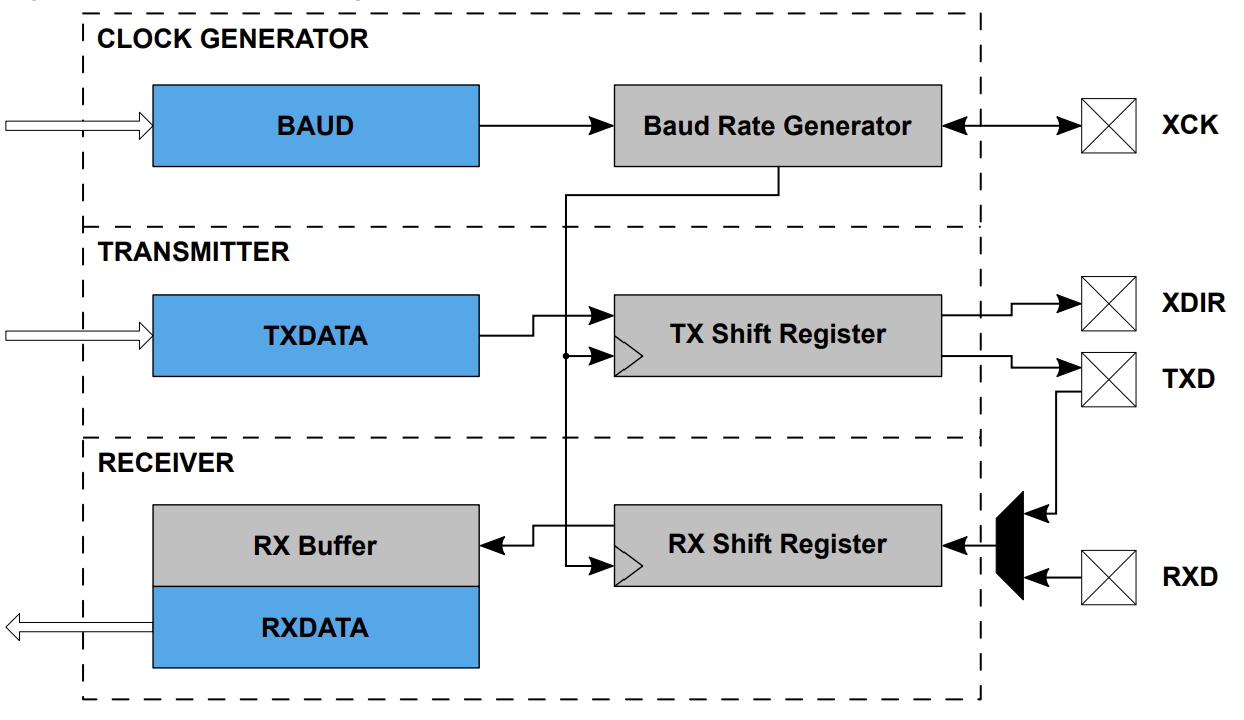
\includegraphics[width=0.85\textwidth]{images/uart_block_diagram.png}
  \caption{UART Block Diagram (Conceptual)}
  \label{fig:uart_blockdiagram}
\end{figure}

\subsection{Top-Level Architecture}
\begin{itemize}
  \item \textbf{APB Interface}: Decodes read/write operations to internal UART registers and FIFOs.
  \item \textbf{TX Path}:
  \begin{itemize}
    \item \textit{TX FIFO}: Buffers data from software.
    \item \textit{UartTx FSM}: Converts parallel data into serial form, inserting start/stop/parity bits.
    \item \textit{Line Driver}: Outputs serial bitstream on the \texttt{tx} pin.
  \end{itemize}
  \item \textbf{RX Path}:
  \begin{itemize}
    \item \textit{UartRx FSM}: Samples the \texttt{rx} line at the correct baud rate. Checks start/stop bits and optional parity.
    \item \textit{RX FIFO}: Buffers received bytes for software to read.
  \end{itemize}
  \item \textbf{Control Registers}: 
    \begin{itemize}
      \item \texttt{clocksPerBitDb}, \texttt{numOutputBitsDb} (for adjustable baud rate and data bits).
      \item FIFO status registers, error flags, etc.
    \end{itemize}
\end{itemize}

\subsection{Clocking and Synchronization}
All logic is synchronous to the APB clock (\texttt{PCLK}). The \texttt{rx} pin is passed through \textit{syncDepth} flip-flops to reduce metastability. The TX path uses the same clock domain and counters to generate appropriate bit timing.

\subsection{Data Flow}
\textbf{Transmit}:
\begin{enumerate}
  \item Software writes bytes to the TX FIFO (by writing \texttt{dataIn} and toggling \texttt{load}).
  \item The transmitter state machine automatically reads from the FIFO when idle and begins sending start bit, data bits, parity (if enabled), and stop bit.
  \item \texttt{txFifoEmpty} goes high once all queued bytes have been sent.
\end{enumerate}

\noindent
\textbf{Receive}:
\begin{enumerate}
  \item The RX logic waits for a start bit (transition from high to low).
  \item Data bits are shifted in at intervals determined by \texttt{clocksPerBitDb}, followed by optional parity and the stop bit.
  \item Completed bytes are pushed into the RX FIFO; software reads them via \texttt{rxData}.
\end{enumerate}
